%%%%%% CMB-S4 Simulations and Data Analysis Chapter, Component Separation Section  %%%%%%%%%%%%%%%%
          
\section{Component Separation}
\label{sec:compsep}

%\textbf{ Authors: Mark Ashdown, Jonathan Aumont, Carlo Baccicalupi, Josquin Errard, Maude Le Jeune}

This section discusses the algorithms and methods for disentangling different sources of sky emission in multi-frequency maps, whether these come exclusively from \cmbexp\ or include well-characterized external maps. Under this assumption, we are able to go beyond simple foreground cleaning to full component separation, which provides both important consistency checks on our results and critical inputs to sky modeling (see below). We first present the motivations and the general ideas of existing approaches. We then give some specifics of parametric and blind methods. Finally, we summarize several questions which might be answered by follow-up studies.

Recent measurements by BICEP2/Keck/\planck\ \cite{Ade:2015tva} confirm that on degree scales, where 
\cmbexp\ is expected to search for 
the imprint of B modes from primordial gravitational waves, the contamination from polarized foreground emission is  comparable to or higher than the cosmological signal at 150~GHz even in one of the cleaner patches of the sky.
Given that 150~GHz is expected to be close to the minimum of foreground contamination vs.~CMB signal, this 
is likely to be the case at all frequencies and all but the smallest fractions of the sky.
Given the power law behavior in $\ell$ found on larger scales by \planck\ and \wmap\ \cite{Adam:2015tpy,Page:2006hz}, foregrounds are expected to be even more relevant at larger angular scales. Foregrounds are expected to be subdominant  with respect to the B-mode lensing signal on the scale of a few arcminutes (see Figure~\ref{fig:power_spectrum_fgs}); nevertheless, dust polarization fractions around $10\%$ (comparable to observed levels) have been shown to have non-negligible impact on the 4-point function used for achieving lensing extraction \cite{Fantaye:2012ha}. Therefore, component separation is a necessary and important step in gaining insight into the amplitude of primordial gravitational waves, the neutrino masses, and the abundance of dark energy through CMB lensing studies.

\begin{figure*}[htbp]
\centering
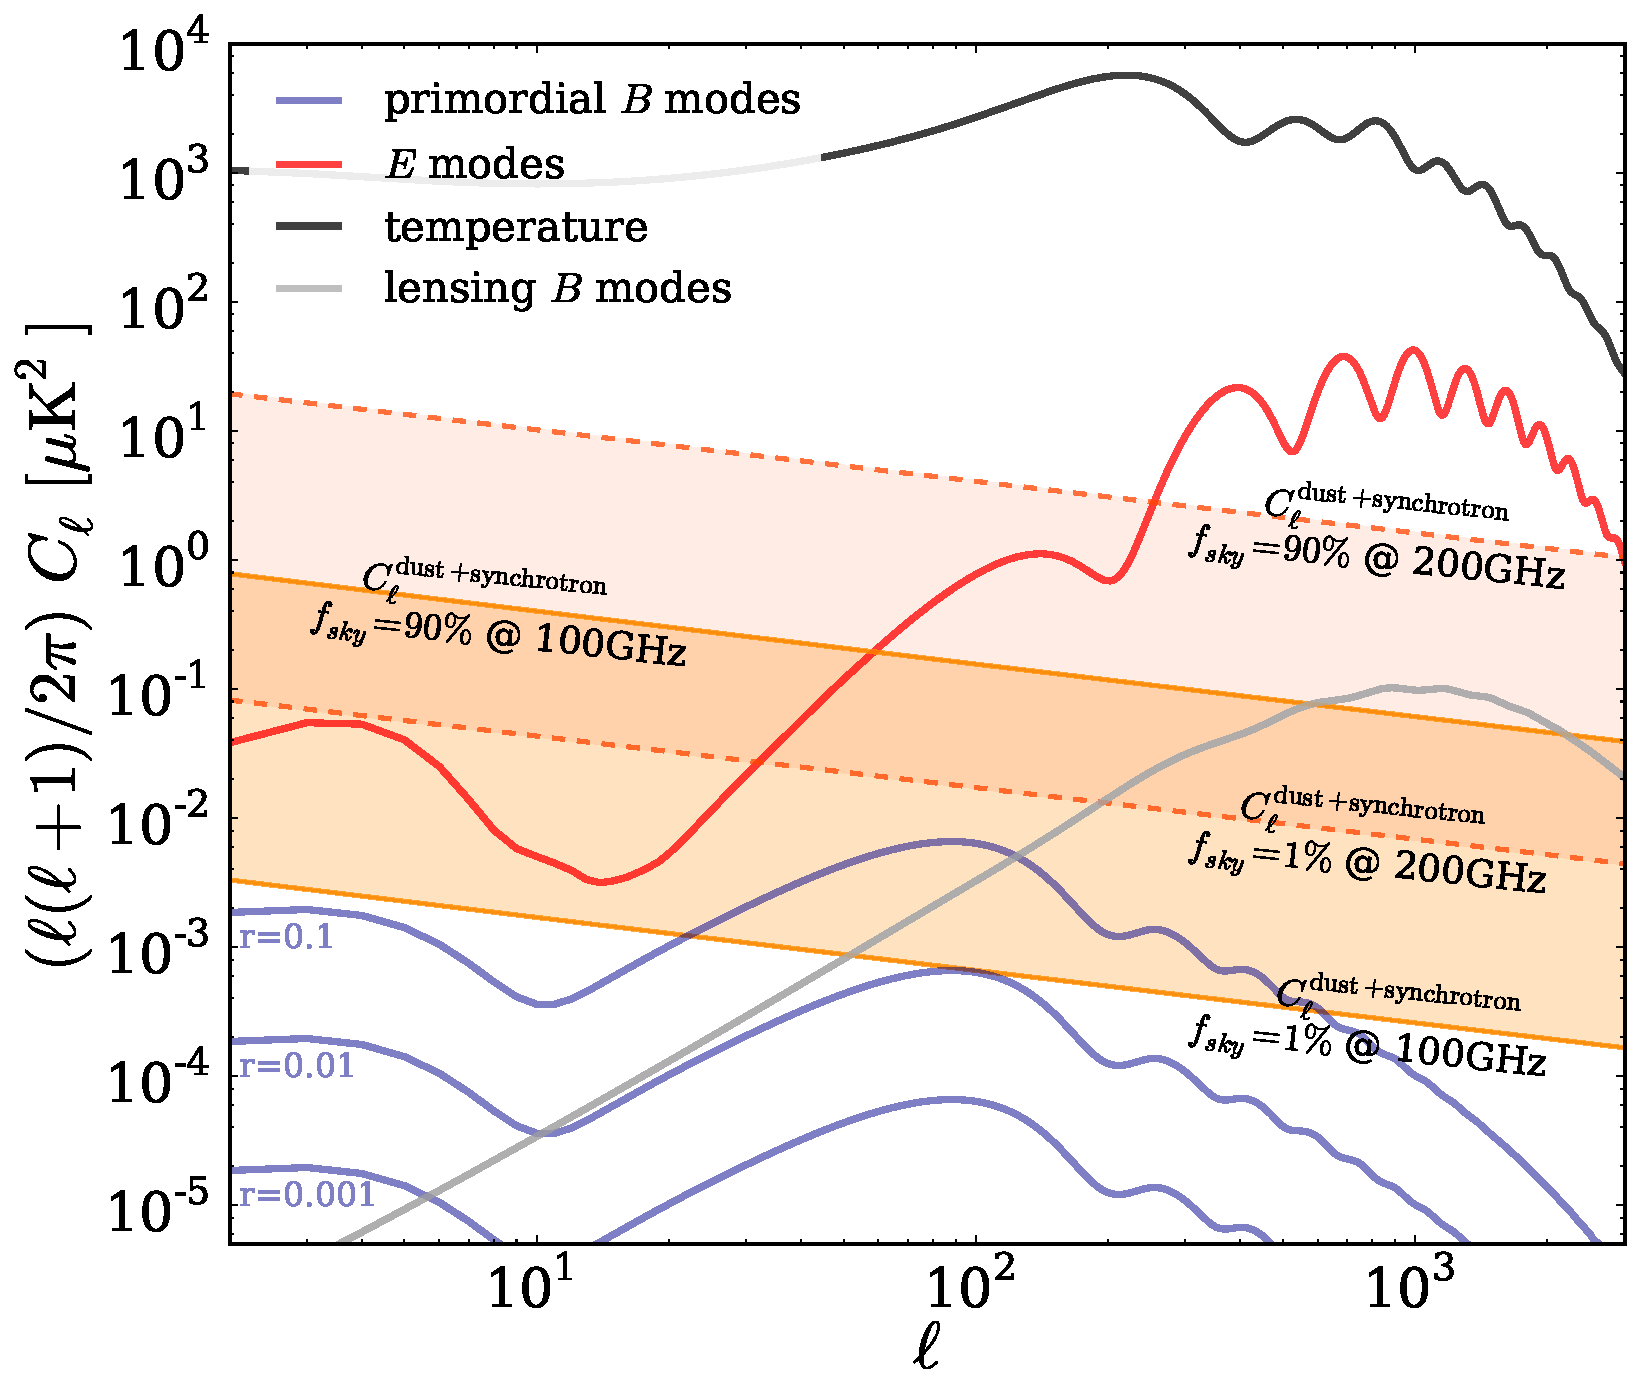
\includegraphics[width=0.5\textwidth]{Analysis/Power_Spectrum_figure_showing_foregrounds.pdf}
\caption{Angular power spectra showing primordial B modes, lensing B modes, total intensity, and E modes, as well as the total contribution of polarized B-mode foregrounds (dust plus synchrotron), expected on the cleanest $1-90\%$ of the sky, at $100$ and $200\;$GHz. Note that these results are derived from \planck\ data on large patches of the sky, and the estimates for 1\% patches of the sky are extrapolations; there may in fact be individual 1\% patches that are cleaner than the levels shown here.
%that, as these results are derived from \planck\ data at intermediate and high Galactic latitudes, sensitive primarily to the large scale 
%foreground pattern in polarization and therefore not optimized for high-resolution, small scale instruments, there is potential for discovery of small patches of sky (e.g., $f_{\mathrm sky} \leq 5\%$) with a signal differing than those indicated here. 
From~\cite{Errard:2015cxa}.}
\label{fig:power_spectrum_fgs}
\end{figure*}

Broadly defined, the process of component separation would generally
\begin{itemize}
	\item include any data processing that characterizes and exploits correlations between observations at multiple frequencies
	\item use external constraints and physical modeling
	\item aim at distinguishing between different physical sources of emission.
\end{itemize}

The general data modeling reads
\begin{eqnarray}
	\centering	
		d_p &=& \sum_{\rm comp, p} a_p^{\rm comp} s^{\rm comp}_p + n_p \equiv \mathbf{A}\,s_p + n_p
	\label{eq:comp_sep_data_modeling}
\end{eqnarray}
where the vector $d_p$ contains the measured signal in each observing band, $\mathbf{A}$ is the so-called mixing matrix which encapsulates the emission law $a_p^{\rm comp}$ of each component, $s_p$ is a vector containing the unknown CMB and foregrounds amplitude, and $n_p$ is a vector containing the noise level at each observing band. The index $p$ refers to sky pixels $\left( \theta, \phi \right)$, or modes of a spherical harmonic decomposition $\left( \ell, m\right)$, or a set of Fourier modes $\left(k_x,k_y\right)$, etc. Note that this modeling assumes spatial templates $s_p$ that are the same in all observing bands.

Component separation aims at inverting Eq.~\ref{eq:comp_sep_data_modeling}, thus estimating the foreground-cleaned CMB signal encapsulated in $s_p$, as well as the foreground maps which are relevant for testing and updating our knowledge of astrophysical processes (and hence improving the sky model).
%, as illustrated in Fig.~\ref{fig:general_comp_sep_scheme}.
The estimate $\tilde{s}_p$ of the true sky templates $s_p$ --- given $\mathbf{A}$, $d_p$ and the statistical properties of the noise --- minimizes the following $\chi^2$:
\begin{eqnarray}
	\centering
		\chi^2 \equiv \sum_p \left| s_p - \tilde{s}_p\right|^2
	\label{eq:chi2_compsep}
\end{eqnarray}
and can be taken to have the following general form
\begin{eqnarray}
	\centering
		\tilde{s}_p = \mathbf{W}\,d_p
	\label{eq:sp_solution}
\end{eqnarray}
where the weighting operator $\mathbf{W}$ is chosen to optimize some criterion regarding $\tilde{s}_p$ and $s_p$ (variance of the cleaned map, unbiasedness, etc.) while keeping statistical consistency and robustness. In particular, a common requirement for all component separation algorithms is the ability of propagating errors due to foreground subtraction, while having the flexibility of including foreground modeling and external constraints in a transparent way. 
Component separation is then defined as a method of estimating the mixing matrix $\mathbf{A}$ and finding the weighting $\mathbf{W}$ that provides closest possible estimate $\tilde{s}_p$ to the true sky signal.

For example, a solution to Eqs.~\ref{eq:chi2_compsep} and~\ref{eq:sp_solution} is obtained by taking $\mathbf{W} \equiv \left( \mathbf{A}^T\mathbf{N}^{-1}\mathbf{A} \right)^{-1}\mathbf{A}^T\mathbf{N}^{-1}$ with $\mathbf{N} \equiv \langle n_p^T n_p\rangle$, leading to an unbiased estimate of the sky. As mentioned below, this expression can be changed (see, e.g., \cite{Delabrouille:2009aa}), depending on the desired level of generality and complexity and on the level of prior knowledge of the sky signal.


Studies have demonstrated the applicability of classes of component separation 
algorithms to certain simulated multi-frequency datasets, either balloon-borne or ground-based, and targeting limited frequency ranges and sky areas \cite{Stivoli:2010rs,Fantaye:2011zq,Fantaye:2012ha}. Results indicate that generally, for a frequency range extending from $90$ to $250$ GHz, polarized foregrounds may be removed effectively through a multi-frequency combination, at the price of enhancing the white noise contribution due to channel mixing; moreover, a possible bias may be introduced if, at the lowest frequency interval edge, the synchrotron component is not negligible: lower frequency templates/data are required to avoid such a contribution \cite{Essinger-Hileman:2014pja}. 
%Along this line, algorithms progressed in terms of casting and analysis to be exploited as a guidance in the optimization of instrumental designs for foreground cleaning \cite{errard11, errard12}, which are now adopted as a standard for forecasting the feasibility of foreground cleaning and impact on the main science targets of B modes \cite{Errard:2015cxa}. 
The most comprehensive application of component separation to data, in terms of completeness of algorithms and frequency range, is represented by \planck\ \cite{Adam:2015tpy}, 
%although dominated by the CMB component  which is accessible by that, i.e. the total intensity and large scale polarization 
although the targeted CMB components in that analysis (total intensity and E-mode polarization) are
not the same as in the \cmbexp\ case.

%%%%%%%%%%%%%%%%%%%%%%
\subsection{Component Separation Methods}

The CMB extraction may be achieved essentially through two basic concepts: the fitting of foreground unknowns along with CMB, or the minimization of the variance of a linear combination of the data, constrained to have the frequency scaling of a blackbody.
The first class of algorithms, known as ``parametric,'' makes the maximum use of prior knowledge of foreground emission. By contrast, the second class, known as ``blind,'' makes the minimum set of assumptions. 
These two broad classes and other possibilities are discussed in turn below.
Both approaches are used widely in the field and have been tested with multiple implementations applied
to multiple data sets. Blind techniques have included those using internal template subtraction (e.g. \cite{Bennett:1992aa,Hansen:2006rj,Katayama:2011eh}) and those exploiting statistical independence of sky components (e.g. \cite{Delabrouille:2002kz,Maino:2006pq,Bonaldi:2006qw,Stolyarov:2004xp}). Implementations of parametric fitting have included the studies in \cite{Brandt:1994aa,Eriksen:2005dr, Stompor:2008sf}.

\begin{itemize}
	\item \textbf{Parametric} -- The overall idea of these methods boils down to two steps: 1) the estimation of the mixing matrix, $\mathbf{A}$; and 2) the inversion of Eq.~\ref{eq:comp_sep_data_modeling} to recover an estimate of the sky signal, $s_p$.
	Parametric methods assumes that the mixing matrix, used in Eq.~\ref{eq:comp_sep_data_modeling}, has a functional form which is known and which can be parametrized by so-called ``spectral'' parameters $\beta$, i.e., $\mathbf{A} = \mathbf{A}(\beta)$. The functional form of $\mathbf{A}$ being fixed, the estimation of the mixing matrix is therefore equivalent to an estimation of the parameters $\beta$. The parameters of the model are determined via a fitting procedure, often performed over sky pixels. This can be achieved by maximizing the following so-called ``spectral" likelihood \cite{Brandt:1994aa,Eriksen:2005dr}:
	\begin{eqnarray}
		\centering
			-2\log \mathcal{L}(\beta) = - \sum_p \left( \mathbf{A}^T\mathbf{N}^{-1} d\right)^T\left( \mathbf{A}^T\mathbf{N}^{-1} \mathbf{A}\right)^{-1}\left( \mathbf{A}^T\mathbf{N}^{-1} d\right).
	\end{eqnarray}
Any deviation between the true mixing matrix $\mathbf{A}$ and the estimated $\mathbf{\tilde A} \equiv A(\tilde \beta)$ leads to the presence of foreground residuals in the reconstructed component maps.
	\item \textbf{Blind} -- Under the  assumption that sky components are statistically independent, blind methods aim to recover these components with an a priori unknown mixing matrix. Blind methods make minimal assumptions about the foregrounds and focus on reconstructing the CMB from its well known blackbody spectral energy distribution. The Internal Linear Combination (ILC, \cite{Tegmark:2003ud}) belongs to this class of methods. It only uses the CMB column of the mixing matrix elements (noted $a$ hereafter) to perform the minimum variance reconstruction, cf. Eq.~\ref{eq:sp_solution}:
\begin{equation}
  \tilde s_p = \sum_{i=0}^{i=m} w_i d_{p,i}
\end{equation}
with $\sum_i  w_i a_i = 1$, leading to the following solution:
\begin{equation}
  w_i = a^T N^{-1} (a^TN^{-1} a)^{-1}
\end{equation}

In this scheme, no attempt is made to design a foreground model. The decorrelation property between CMB and foregrounds alone is used to project out the contamination into a $m$-1 subspace (with $m$ being the number of frequency maps).

The main caveat in this method is its well known bias (\cite{Hinshaw:2006ia, Delabrouille:2009aa}, etc) which comes from empirical correlation between the CMB and the foregrounds. The ILC bias is proportional to the number of detectors $m$ and inversely proportional to the number of pixels used to compute $N$. In order to reduce this effect, one could think of reducing the foreground subspace size by adding further constraints. The SEVEM template fitting method (\cite{MartinezGonzalez:2003dy}, etc) follows this idea, by building some foreground templates with a combination of a subset of the input frequency maps.

The semi-blind SMICA method~\cite{Cardoso:2008qt} also works at containing the foreground in a smaller dimension space, but in a more general way. The idea of Independent Component Analysis (ICA) is to blindly recover the full mixing matrix $\mathbf{A}$ by using the independence property of the different components. As we know that they are spatial correlations between the foregrounds, the ICA principle is used to disentangle the CMB from the noise and the foregrounds taken as a whole.

The main advantage of such blind or semi-blind methods is their ability to face any unknown and/or complex foreground contamination, to reconstruct a clean CMB signal. This is a big advantage when real data comes, one can then focus on instrumental effects, or data set combination issues at first, and leave the complex task of the foreground modeling and reconstruction for a future analysis step.

Moreover, in a framework like SMICA, the level of blindness can be adjusted via the plugin of any parametric component to its flexible engine as described in~\cite{Cardoso:2008qt}, allowing for a step by step fine grain design of the foreground model.\\
	%\item \textbf{Maximum entropy} --  this is a method which inverts the same linear system of component mixtures, cf Eq.~\ref{eq:comp_sep_data_modeling}, but assumes non-gaussian probability distributions, see \cite{hobson98,stolyarov02}. Yet, the introduced prior for this particular approach biases the reconstruction of the components, especially weak ones, which will not be suitable for CMB polarisation characterization.
	\item \textbf{Template fitting} -- 	In this variant, emission laws are not modeled, and the analysis is reduced to the maximisation of a likelihood over 
%scalar and tensor contributions to any CMB angular power spectrum, as well as 
the CMB contribution and the amplitudes of each foreground component (see, e.g., \cite{Katayama:2011eh}).
\end{itemize}

%Discussion regarding the domain of application (harmonic, pixel, wavelet, etc.)} -- t
For all of the approaches discussed above, Eq.~\ref{eq:sp_solution} can be implemented equivalently with any representations of the map---i.e. pixel, harmonic, wavelet, etc. The resulting component separation is independent of this choice as long as the linear data modeling (Eq.~\ref{eq:comp_sep_data_modeling}) holds. 
This complementarity, and the internal comparison of results through these pipelines has been proven to be relevant in actual analysis of \planck\ data \cite{Adam:2015tpy}. That said, the difference between domain of application will lie in the computational needs: for high number of sky pixels, the implementation of Eq.~\ref{eq:sp_solution} might be significantly more efficient in harmonic space. 
%Both can be cast in the default, spatial domain of sky pixels, as well as a variety of harmonic domains, extending from the pure angular one, to the selection of localization in the spatial and harmonic domains through a suitable needlet set. This complementarity, and the internal comparison of results through these pipelines has been proven to be relevant in actual analysis of \planck\ data \cite{Adam:2015tpy}. 

One practical difference of particular interest between these approaches is how uncertainties in the 
foreground model get propagated to uncertainties in data products derived from the foreground-cleaned
maps, such as angular power spectra and cosmological parameters. In parametric models, any statistical 
covariance between foreground parameters and the cleaned CMB is properly captured (at the 
Gaussian-approximation level) in the resulting covariance matrix. For non-parametric methods, this 
covariance can be approximated using Monte Carlo methods, which can be problematic for foregrounds
on the largest scales, the distribution of which is quite clearly non-Gaussian. This issue is discussed further
in Section~\ref{se:challenges}.

%\textcolor{red}{JE: $\rightarrow$ Parametric fitting vs. ILC, spatial domain versus non-spatial, that makes a basis of 4 algorithms. Although it was never quantified, the independence of those and very different hypotheses represent an opportunity for cross-checking and robustness.}

%%%%%%%%%%%%%%%%%%%%%%
\subsection{Open Questions}
\begin{itemize}
	\item \textbf{E/B or Q/U basis of analysis} -- Component separation between CMB radiation and its foregrounds can be performed either dealing with Stokes parameters $Q$ and $U$ maps of the sky in real space or Fourier space, and either before or after the separation between the E and B modes. Several approaches have been followed by CMB experiments so far \cite{Gold:2010fm,Aghanim:2015xee, Ade:2015tva},
%(see e.g. \cite{Gold:2010fm,Aghanim:2015xee} for real space and e.g \cite{Ade:2015tva} for Fourier space separations) 
and each of them has some advantages and some caveats. For example, processing $Q/U$ data in the map domain 
%allows to preserve all the informations on the foreground components that have non-Gaussian spatial distributions 
simplifies the treatment of foreground components that have non-Gaussian and/or non-stationary
spatial distributions.
%and/or exploit them to disentangle efficiently Galactic and cosmological signals. 
However, in the $Q$ and $U$ basis, the CMB E and B modes are mixed and the CMB E modes will be the dominant contribution to the variance at intermediate and small scales in the CMB observing frequencies, limiting the accuracy of the separation.
%from foregrounds. 
To overcome this limitation, E and B observables can be constructed in Fourier space. 
%On the cut sky (because even if the full sky could be observed, some of the brightest foreground emitting regions near the Galactic center have to be masked out), this separation implies an additional variance (known as the E to B leakage), which might be significant even after correction and on large fractions of the sky, when trying to measure the CMB B modes for $r\simeq10^{-3}$ \cite{ferte13}. 
The separation of the B-mode components (primordial CMB, Galactic foregrounds, lensing, etc.) can then be done in the angular power spectrum domain (where the final accuracy might be limited by the cosmic variance associated to foregrounds),
%, orders of magnitude larger than the primordial CMB B-modes) 
in the two-dimensional, phase-full Fourier domain (where the treatment of non-stationary components
will be complicated) or in the map domain (where the final accuracy might be limited by ringing of the foregrounds due to the non-local transformation). 
%While for $Q$ and $U$ the problem we face is analogous in terms of foreground vs CMB balance, for E and B that is not: E is more similar to $Q$ and $U$, but in the B channel separation is more challenging. We have the capability and will analyze in both domains, to validate and cross-check the stability of the mixing matrix recovery.
Although these different approaches are currently giving satisfactory results on simulated data, these effects will become crucial at the sensitivity of \cmbexp\ and merit a dedicated study. 
	\item \textbf{Combining data from multiple instruments} -- Ground-based instruments heavily filter time streams because of atmosphere contamination, ground emission, etc. %to perform projections on the sky. 
	In particular, large angular scales are usually suppressed anisotropically, and this suppression is corrected in the power spectrum estimate. 
%	In order to perform component separation using various observations, component separation methods will require the use of maps derived from common filters. \\
Component separation using observations from different platforms will be made more straightforward if all maps are derived from common filters. 
As stressed already, the first attempt at component separation or foreground cleaning for  B modes on multi-platform data was recently implemented in \cite{Ade:2015tva}, using data from BICEP2, Keck Array and \planck. A template fitting analysis was implemented with the primary objective of minimizing the variance in the CMB solution.%, by achieving a linear combination of the data, which turned out in a reduction of the power observed from the ground, which is interpreted as cleaning of the Galactic dust, and sets the current limit on B modes from primordial GWs. 
%The independent reduction of the data 
The simultaneous analysis of combined data sets 
required an additional layer in the analysis, namely the simulated scans of the \planck\ data through the filtering by the ground observatories, along with validation through simulations of the whole procedure. A simpler approach for \cmbexp\ would be to have a single pipeline reducing and combining different datasets. With a common filtering implemented from scratch in a multi-site experiment, the %latter a posteriori 
combination would be built-in, thus avoiding the extra layer and increasing confidence and robustness of results.
	\item \textbf{Various resolutions} -- Under the approximation that the mixing matrix does not significantly vary as a function of resolution, the impact of different beam sizes can be propagated to the noise level of the final CMB map %through the CMB x CMB term of $\left(\mathbf{A}^T\mathbf{N}^{-1}\mathbf{A}\right)^{-1}$ as given by Eq.~\ref{eq:sp_solution} with $\mathbf{W} \equiv \left( \mathbf{A}^T\mathbf{N}^{-1}\mathbf{A} \right)^{-1}\mathbf{A}^T\mathbf{N}^{-1}$. 
by incorporating the beam for each frequency channel in the expression of the noise covariance matrix 
	\begin{eqnarray}
		\centering
			\mathbf{N}(i) \equiv \mathbf{N}(i)_\ell = \left( \sigma_i\right)^2\exp\left[ \frac{\ell(\ell+1)\theta_{\rm FWHM}^2}{8\log(2)} \right]
	\end{eqnarray}
	where $i$ is a frequency channel and $\sigma_i$ is the noise level in the corresponding map. The noise variance in the reconstructed CMB map, i.e. after component separation, would then be given by
	\begin{eqnarray}
		\centering
			N_\ell^{\rm post\ comp\ sep} = \left[\left(\mathbf{A}^T\left(\mathbf{N}_\ell\right)^{-1}\mathbf{A}\right)^{-1}\right]_{\rm CMBxCMB}.
	\end{eqnarray}
%	The effective beam of this noise is degraded compared to a simple quadratically combined noise, but this obviously depends on the involved beams sizes and on the importance of given channels to perform the foregrounds cleaning.
	\item \textbf{Atmosphere residuals} -- Atmosphere residuals appear at large scales in ground-based CMB observations, and they scale with frequency in a similar way as dust, $\propto \nu^\beta$ \cite{Errard:2015twg}. Having redundant frequencies among the different observatories could help mitigate the atmospheric and astrophysical foregrounds. Furthermore, the small intrinsic polarization of the atmosphere \cite{Battistelli:2012we,Errard:2015twg} will
limit the contamination to component separation of the polarized signals.
Still, this effect will have to be investigated quantitatively with realistic simulations.
\end{itemize}

%\textcolor{red}{JE: we could outline a roadmap, i.e. the application and learning phase to SIV made by the various sub-orbitals which are going on-line now or soon with the usual 95, 150, 220. That would need to be investigated very accurately as it would represent a most important step for component separation towards SIV.}



%\bibliography{cmbs4}

%%
%% Populate the .bib file with entries from SPIRES Bibtex (preferred)
%% or ADS Bibtex (if no SPIRES entry).
%%  SPIRES will also supply the CITATION line information; please include it.
%%
